%!TEX program = xelatex

\documentclass[a4paper, openany, oneside]{memoir}
\usepackage[no-math]{fontspec}
\usepackage{pgfplots}
\pgfplotsset{compat=newest}
\usepackage{commath}
\usepackage{mathtools}
\usepackage{amssymb}
\usepackage{amsthm}
\usepackage{booktabs}
\usepackage{mathtools}
\usepackage{xcolor}
\usepackage[separate-uncertainty=true, per-mode=symbol]{siunitx}
\usepackage[noabbrev, capitalize]{cleveref}
\usepackage{listings}
\usepackage[american inductor, european resistor]{circuitikz}
\usepackage{amsmath}
\usepackage{amsfonts}
\usepackage{ifxetex}
\usepackage[dutch,english]{babel}
\usepackage[backend=bibtexu,texencoding=utf8,bibencoding=utf8,style=ieee,sortlocale=en_GB,language=auto]{biblatex}
\usepackage[strict,autostyle]{csquotes}
\usepackage{parskip}
\usepackage{import}
\usepackage{standalone}
\usepackage{hyperref}
%\usepackage[toc,title,titletoc]{appendix}

\ifxetex{} % Fonts laden in het geval dat je met Xetex compiled
    \usepackage{fontspec}
    \defaultfontfeatures{Ligatures=TeX} % To support LaTeX quoting style
    \setromanfont{Palatino Linotype} % Tover ergens in Font mapje in root.
    \setmonofont{Source Code Pro}
\else % Terug val in standaard pdflatex tool chain. Geen ondersteuning voor OTT fonts
    \usepackage[T1]{fontenc}
    \usepackage[utf8]{inputenc}
\fi
\newcommand{\references}[1]{\begin{flushright}{#1}\end{flushright}}
\renewcommand{\vec}[1]{\boldsymbol{\mathbf{#1}}}
\newcommand{\uvec}[1]{\boldsymbol{\hat{\vec{#1}}}}
\newcommand{\mat}[1]{\boldsymbol{\mathbf{#1}}}
\newcommand{\fasor}[1]{\boldsymbol{\tilde{\vec{#1}}}}
\newcommand{\cmplx}[0]{\mathrm{j}}
\renewcommand{\Re}[0]{\operatorname{Re}}
\newcommand{\Cov}{\operatorname{Cov}}
\newcommand{\Var}{\operatorname{Var}}
\newcommand{\proj}{\operatorname{proj}}
\newcommand{\Perp}{\operatorname{perp}}
\newcommand{\col}{\operatorname{col}}
\newcommand{\rect}{\operatorname{rect}}
\newcommand{\sinc}{\operatorname{sinc}}
\newcommand{\IT}{\operatorname{IT}}
\newcommand{\F}{\mathcal{F}}

\newtheorem{definition}{Definition}
\newtheorem{theorem}{Theorem}


\DeclareSIUnit{\voltampere}{VA} %apparent power
\DeclareSIUnit{\pii}{\ensuremath{\pi}}

\hypersetup{%setup hyperlinks
    colorlinks,
    citecolor=black,
    filecolor=black,
    linkcolor=black,
    urlcolor=black
}

% Example boxes
\usepackage{fancybox}
\usepackage{framed}
\usepackage{adjustbox}
\newenvironment{simpages}%
{\AtBeginEnvironment{itemize}{\parskip=0pt\parsep=0pt\partopsep=0pt}
\def\FrameCommand{\fboxsep=.5\FrameSep\shadowbox}\MakeFramed{\FrameRestore}}%
{\endMakeFramed}

% Impulse train
\DeclareFontFamily{U}{wncy}{}
\DeclareFontShape{U}{wncy}{m}{n}{<->wncyr10}{}
\DeclareSymbolFont{mcy}{U}{wncy}{m}{n}
\DeclareMathSymbol{\Sha}{\mathord}{mcy}{"58}
\addbibresource{../../../../includes/bibliography.bib}

\begin{document}

\subsection{Coprime sampling}\label{sec:coprime}
As we argued before, the algorithm design in \cref{cha:reconstruction} is not designed to process two signals sampled by coprime sampling. This yields that some preprocessing is necessary. The idea is to break the signal sampled by coprime sampling into many different signals which seem to be sampled uniformly. More specifically, we break the signals of the two different samplers with sampling periods $aT$ and $bT$ into artificial signals with sampling period $abT$. This is illustrated in \cref{tkz:sc_coprime,tkz:pre-coprime}.

\begin{figure}
\centerline{
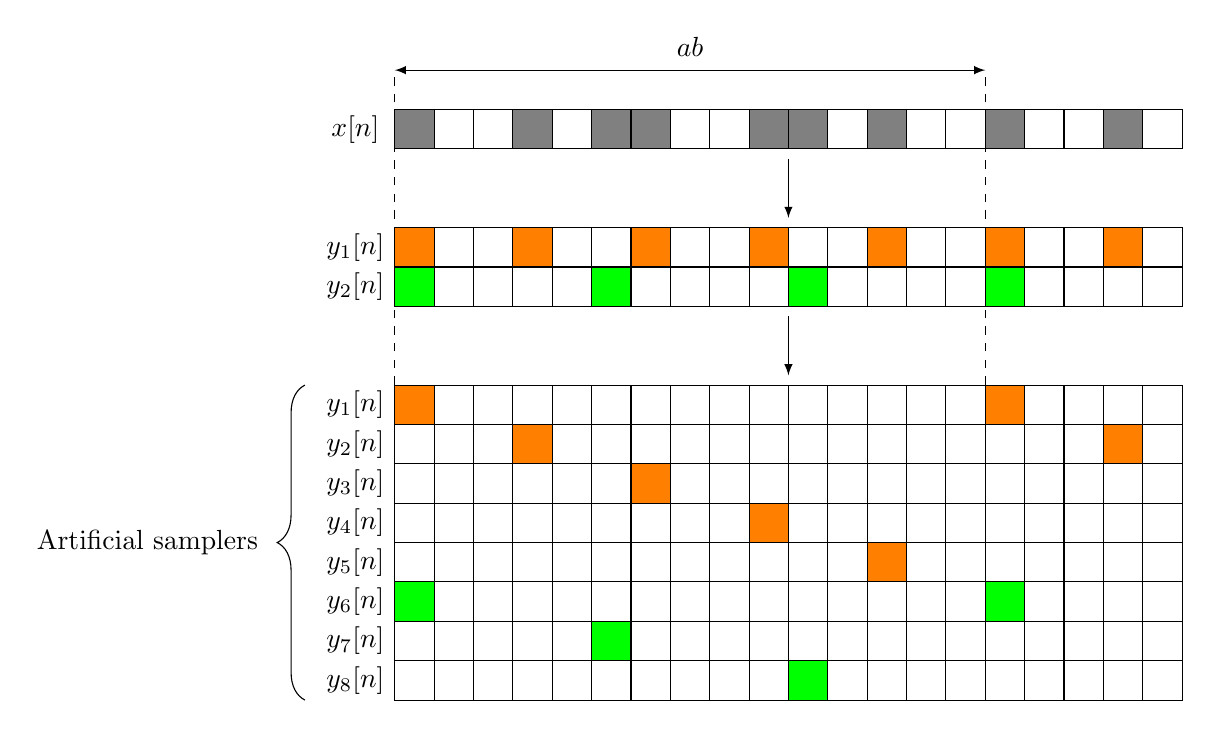
\begin{tikzpicture}
\draw  [fill=gray](-1.5,0.5) rectangle (-1,0);
\draw  (-1,0.5) rectangle (-0.5,0);
\draw  (-0.5,0.5) rectangle (0,0);
\draw  [fill=gray](0,0.5) rectangle (0.5,0);
\draw  (0.5,0.5) rectangle (1,0);
\draw  [fill=gray](1,0.5) rectangle (1.5,0);
\draw  [fill=gray](1.5,0.5) rectangle (2,0);
\draw  (2,0.5) rectangle (2.5,0);
\draw  (2.5,0.5) rectangle (3,0);
\draw  [fill=gray](3,0.5) rectangle (3.5,0);
\draw [fill=gray] (3.5,0.5) rectangle (4,0);
\draw  (4,0.5) rectangle (4.5,0);
\draw  [fill=gray](4.5,0.5) rectangle (5,0);
\draw  (5,0.5) rectangle (5.5,0);
\draw  (5.5,0.5) rectangle (6,0);
\draw [fill=gray](6,0.5) rectangle (6.5,0);
\draw  (6.5,0.5) rectangle (7,0);
\draw  (7,0.5) rectangle (7.5,0);
\draw  [fill=gray](7.5,0.5) rectangle (8,0);
\draw  (8,0.5) rectangle (8.5,0);
\draw  [fill=orange](-1.5,-1) rectangle (-1,-1.5);
\draw  (-1,-1) rectangle (-0.5,-1.5);
\draw  (-0.5,-1) rectangle (0,-1.5);
\draw  [fill=orange](0,-1) rectangle (0.5,-1.5);
\draw  (0.5,-1) rectangle (1,-1.5);
\draw  (1,-1) rectangle (1.5,-1.5);
\draw  [fill=orange](1.5,-1) rectangle (2,-1.5);
\draw  (2,-1) rectangle (2.5,-1.5);
\draw  (2.5,-1) rectangle (3,-1.5);
\draw  [fill=orange](3,-1) rectangle (3.5,-1.5);
\draw  (3.5,-1) rectangle (4,-1.5);
\draw  (4,-1) rectangle (4.5,-1.5);
\draw  [fill=orange](4.5,-1) rectangle (5,-1.5);
\draw  (5,-1) rectangle (5.5,-1.5);
\draw  (5.5,-1) rectangle (6,-1.5);
\draw  [fill=orange](6,-1) rectangle (6.5,-1.5);
\draw  (6.5,-1) rectangle (7,-1.5);
\draw  (7,-1) rectangle (7.5,-1.5);
\draw  [fill=orange](7.5,-1) rectangle (8,-1.5);
\draw  (8,-1) rectangle (8.5,-1.5);
\draw  [fill=green](-1.5,-1.5) rectangle (-1,-2);
\draw  (-1,-1.5) rectangle (-0.5,-2);
\draw  (-0.5,-1.5) rectangle (0,-2);
\draw  (0,-1.5) rectangle (0.5,-2);
\draw  (0.5,-1.5) rectangle (1,-2);
\draw [fill=green] (1,-1.5) rectangle (1.5,-2);
\draw  (1.5,-1.5) rectangle (2,-2);
\draw  (2,-1.5) rectangle (2.5,-2);
\draw  (2.5,-1.5) rectangle (3,-2);
\draw  (3,-1.5) rectangle (3.5,-2);
\draw  [fill=green](3.5,-1.5) rectangle (4,-2);
\draw  (4,-1.5) rectangle (4.5,-2);
\draw  (4.5,-1.5) rectangle (5,-2);
\draw  (5,-1.5) rectangle (5.5,-2);
\draw  (5.5,-1.5) rectangle (6,-2);
\draw [fill=green] (6,-1.5) rectangle (6.5,-2);
\draw  (6.5,-1.5) rectangle (7,-2);
\draw  (7,-1.5) rectangle (7.5,-2);
\draw  (7.5,-1.5) rectangle (8,-2);
\draw  (8,-1.5) rectangle (8.5,-2);
\draw  [fill=orange](-1.5,-3) rectangle (-1,-3.5);
\draw  (-1,-3) rectangle (-0.5,-3.5);
\draw  (-0.5,-3) rectangle (0,-3.5);
\draw  (0,-3) rectangle (0.5,-3.5);
\draw  (0.5,-3) rectangle (1,-3.5);
\draw  (1,-3) rectangle (1.5,-3.5);
\draw  (1.5,-3) rectangle (2,-3.5);
\draw  (2,-3) rectangle (2.5,-3.5);
\draw  (2.5,-3) rectangle (3,-3.5);
\draw  (3,-3) rectangle (3.5,-3.5);
\draw  (3.5,-3) rectangle (4,-3.5);
\draw  (4,-3) rectangle (4.5,-3.5);
\draw  (4.5,-3) rectangle (5,-3.5);
\draw  (5,-3) rectangle (5.5,-3.5);
\draw  (5.5,-3) rectangle (6,-3.5);
\draw  [fill=orange](6,-3) rectangle (6.5,-3.5);
\draw  (6.5,-3) rectangle (7,-3.5);
\draw  (7,-3) rectangle (7.5,-3.5);
\draw  (7.5,-3) rectangle (8,-3.5);
\draw  (8,-3) rectangle (8.5,-3.5);
\draw  (-1.5,-3.5) rectangle (-1,-4);
\draw  (-1,-3.5) rectangle (-0.5,-4);
\draw  (-0.5,-3.5) rectangle (0,-4);
\draw  [fill=orange](0,-3.5) rectangle (0.5,-4);
\draw  (0.5,-3.5) rectangle (1,-4);
\draw  (1,-3.5) rectangle (1.5,-4);
\draw  (1.5,-3.5) rectangle (2,-4);
\draw  (2,-3.5) rectangle (2.5,-4);
\draw  (2.5,-3.5) rectangle (3,-4);
\draw  (3,-3.5) rectangle (3.5,-4);
\draw  (3.5,-3.5) rectangle (4,-4);
\draw  (4,-3.5) rectangle (4.5,-4);
\draw  (4.5,-3.5) rectangle (5,-4);
\draw  (5,-3.5) rectangle (5.5,-4);
\draw  (5.5,-3.5) rectangle (6,-4);
\draw  (6,-3.5) rectangle (6.5,-4);
\draw  (6.5,-3.5) rectangle (7,-4);
\draw  (7,-3.5) rectangle (7.5,-4);
\draw  [fill=orange](7.5,-3.5) rectangle (8,-4);
\draw  (8,-3.5) rectangle (8.5,-4);
\draw  (-1.5,-4) rectangle (-1,-4.5);
\draw  (-1,-4) rectangle (-0.5,-4.5);
\draw  (-0.5,-4) rectangle (0,-4.5);
\draw  (0,-4) rectangle (0.5,-4.5);
\draw  (0.5,-4) rectangle (1,-4.5);
\draw  (1,-4) rectangle (1.5,-4.5);
\draw  [fill=orange](1.5,-4) rectangle (2,-4.5);
\draw  (2,-4) rectangle (2.5,-4.5);
\draw  (2.5,-4) rectangle (3,-4.5);
\draw  (3,-4) rectangle (3.5,-4.5);
\draw  (3.5,-4) rectangle (4,-4.5);
\draw  (4,-4) rectangle (4.5,-4.5);
\draw  (4.5,-4) rectangle (5,-4.5);
\draw  (5,-4) rectangle (5.5,-4.5);
\draw  (5.5,-4) rectangle (6,-4.5);
\draw  (6,-4) rectangle (6.5,-4.5);
\draw  (6.5,-4) rectangle (7,-4.5);
\draw  (7,-4) rectangle (7.5,-4.5);
\draw  (7.5,-4) rectangle (8,-4.5);
\draw  (8,-4) rectangle (8.5,-4.5);
\draw (-1.5,-4.5) rectangle (-1,-5);
\draw  (-1,-4.5) rectangle (-0.5,-5);
\draw  (-0.5,-4.5) rectangle (0,-5);
\draw (0,-4.5) rectangle (0.5,-5);
\draw  (0.5,-4.5) rectangle (1,-5);
\draw  (1,-4.5) rectangle (1.5,-5);
\draw  (1.5,-4.5) rectangle (2,-5);
\draw  (2,-4.5) rectangle (2.5,-5);
\draw  (2.5,-4.5) rectangle (3,-5);
\draw  [fill=orange](3,-4.5) rectangle (3.5,-5);
\draw  (3.5,-4.5) rectangle (4,-5);
\draw  (4,-4.5) rectangle (4.5,-5);
\draw (4.5,-4.5) rectangle (5,-5);
\draw  (5,-4.5) rectangle (5.5,-5);
\draw  (5.5,-4.5) rectangle (6,-5);
\draw  (6,-4.5) rectangle (6.5,-5);
\draw  (6.5,-4.5) rectangle (7,-5);
\draw  (7,-4.5) rectangle (7.5,-5);
\draw  (7.5,-4.5) rectangle (8,-5);
\draw  (8,-4.5) rectangle (8.5,-5);
\draw  (-1.5,-5) rectangle (-1,-5.5);
\draw  (-1,-5) rectangle (-0.5,-5.5);
\draw  (-0.5,-5) rectangle (0,-5.5);
\draw  (0,-5) rectangle (0.5,-5.5);
\draw  (0.5,-5) rectangle (1,-5.5);
\draw  (1,-5) rectangle (1.5,-5.5);
\draw  (1.5,-5) rectangle (2,-5.5);
\draw  (2,-5) rectangle (2.5,-5.5);
\draw  (2.5,-5) rectangle (3,-5.5);
\draw  (3,-5) rectangle (3.5,-5.5);
\draw  (3.5,-5) rectangle (4,-5.5);
\draw  (4,-5) rectangle (4.5,-5.5);
\draw  [fill=orange](4.5,-5) rectangle (5,-5.5);
\draw  (5,-5) rectangle (5.5,-5.5);
\draw  (5.5,-5) rectangle (6,-5.5);
\draw  (6,-5) rectangle (6.5,-5.5);
\draw  (6.5,-5) rectangle (7,-5.5);
\draw  (7,-5) rectangle (7.5,-5.5);
\draw  (7.5,-5) rectangle (8,-5.5);
\draw  (8,-5) rectangle (8.5,-5.5);
\draw  [fill=green](-1.5,-5.5) rectangle (-1,-6);
\draw  (-1,-5.5) rectangle (-0.5,-6);
\draw  (-0.5,-5.5) rectangle (0,-6);
\draw  (0,-5.5) rectangle (0.5,-6);
\draw  (0.5,-5.5) rectangle (1,-6);
\draw  (1,-5.5) rectangle (1.5,-6);
\draw  (1.5,-5.5) rectangle (2,-6);
\draw  (2,-5.5) rectangle (2.5,-6);
\draw  (2.5,-5.5) rectangle (3,-6);
\draw  (3,-5.5) rectangle (3.5,-6);
\draw  (3.5,-5.5) rectangle (4,-6);
\draw  (4,-5.5) rectangle (4.5,-6);
\draw  (4.5,-5.5) rectangle (5,-6);
\draw  (5,-5.5) rectangle (5.5,-6);
\draw  (5.5,-5.5) rectangle (6,-6);
\draw [fill=green] (6,-5.5) rectangle (6.5,-6);
\draw  (6.5,-5.5) rectangle (7,-6);
\draw  (7,-5.5) rectangle (7.5,-6);
\draw  (7.5,-5.5) rectangle (8,-6);
\draw  (8,-5.5) rectangle (8.5,-6);
\draw  (-1.5,-6) rectangle (-1,-6.5);
\draw  (-1,-6) rectangle (-0.5,-6.5);
\draw  (-0.5,-6) rectangle (0,-6.5);
\draw  (0,-6) rectangle (0.5,-6.5);
\draw  (0.5,-6) rectangle (1,-6.5);
\draw [fill=green] (1,-6) rectangle (1.5,-6.5);
\draw  (1.5,-6) rectangle (2,-6.5);
\draw  (2,-6) rectangle (2.5,-6.5);
\draw  (2.5,-6) rectangle (3,-6.5);
\draw  (3,-6) rectangle (3.5,-6.5);
\draw  (3.5,-6) rectangle (4,-6.5);
\draw  (4,-6) rectangle (4.5,-6.5);
\draw  (4.5,-6) rectangle (5,-6.5);
\draw  (5,-6) rectangle (5.5,-6.5);
\draw  (5.5,-6) rectangle (6,-6.5);
\draw  (6,-6) rectangle (6.5,-6.5);
\draw  (6.5,-6) rectangle (7,-6.5);
\draw  (7,-6) rectangle (7.5,-6.5);
\draw  (7.5,-6) rectangle (8,-6.5);
\draw  (8,-6) rectangle (8.5,-6.5);
\draw  (-1.5,-6.5) rectangle (-1,-7);
\draw  (-1,-6.5) rectangle (-0.5,-7);
\draw  (-0.5,-6.5) rectangle (0,-7);
\draw  (0,-6.5) rectangle (0.5,-7);
\draw  (0.5,-6.5) rectangle (1,-7);
\draw  (1,-6.5) rectangle (1.5,-7);
\draw  (1.5,-6.5) rectangle (2,-7);
\draw  (2,-6.5) rectangle (2.5,-7);
\draw  (2.5,-6.5) rectangle (3,-7);
\draw  (3,-6.5) rectangle (3.5,-7);
\draw  [fill=green](3.5,-6.5) rectangle (4,-7);
\draw  (4,-6.5) rectangle (4.5,-7);
\draw  (4.5,-6.5) rectangle (5,-7);
\draw  (5,-6.5) rectangle (5.5,-7);
\draw  (5.5,-6.5) rectangle (6,-7);
\draw  (6,-6.5) rectangle (6.5,-7);
\draw  (6.5,-6.5) rectangle (7,-7);
\draw  (7,-6.5) rectangle (7.5,-7);
\draw  (7.5,-6.5) rectangle (8,-7);
\draw  (8,-6.5) rectangle (8.5,-7);
\node (v1) at (3.5,0) {};
\node (v2) at (3.5,-1) {};
\draw  [>=latex,->](v1) edge (v2);
\node (v3) at (3.5,-2) {};
\node (v4) at (3.5,-3) {};
\draw  [>=latex,->](v3) edge (v4);
\draw (-2,0.25) node {$x[n]$};
\draw (-2,0.25-1.5) node {$y_1[n]$};
\draw (-2,0.25-1.5-0.5) node {$y_2[n]$};
\draw (-2,0.25-3.5) node {$y_1[n]$};
\draw (-2,0.25-3.5-0.5) node {$y_2[n]$};
\draw (-2,0.25-3.5-1) node {$y_3[n]$};
\draw (-2,0.25-3.5-1.5) node {$y_4[n]$};
\draw (-2,0.25-3.5-2) node {$y_5[n]$};
\draw (-2,0.25-3.5-2.5) node {$y_6[n]$};
\draw (-2,0.25-3.5-3) node {$y_7[n]$};
\draw (-2,0.25-3.5-3.5) node {$y_8[n]$};
\draw [decorate,decoration={brace,amplitude=10pt},xshift=-4pt,yshift=0pt]
(-2.5,-4.5-4.5+2) -- (-2.5,-0.5-4.5+2) node [black,midway,xshift=-2cm] 
{Artificial samplers};
\draw [dashed](-1.5,-7) -- (-1.5,1);
\draw [dashed](-1.5+6+1.5,-7) -- (-1.5+6+1.5,1);
\draw [>=latex,<->] (-1.5,1) -- node[yshift=0.3cm] {$ab$} (-1.5+6+1.5,1);
\end{tikzpicture}}
\caption{Preproccesing of a signal sampled by coprime sampling}\label{tkz:pre-coprime}
\end{figure}

In \cref{tkz:pre-coprime}, the grey blocks represent the samples recovered by the coprime sampling device. The orange blocks represent the samples that are recoverd by the sampler with sampling period $aT$, and the green blocks represent the samples that are recovered by the sampler with sampling period $bT$. Finally, the bottom block shows how the the orange and greens blocks are split across many artificial signals. These artificial signals represent samplers with an uniform sampling period. Therefore, these artificial samplers make reconstruction possible.

Coprime sampling is dicussed more carefully in \cref{ap:circ-ruler}.
\end{document}
